\chapter{Conception Fine et Réalisation Technique}

\section{Pipeline ETL et Préparation des Données (etl\_HR.pbix)}
La phase ETL a été conçue pour transformer des données RH brutes et hétérogènes en un ensemble cohérent et prêt pour l'analyse.

\subsection{Transformations appliquées sous Power Query}
Les principales étapes de transformation incluent :
\begin{itemize}
    \item \textbf{Typage et Nettoyage :} Conversion des colonnes de salaire en entier et normalisation des noms de départements.
    \item \textbf{Gestion des valeurs nulles :} Pour les employés actifs, la date de sortie (\textit{ExitDate}) a été gérée dynamiquement pour permettre le calcul de l'ancienneté.
    \item \textbf{Segmentation (SalaryBand) :} Création d'une colonne conditionnelle classant les employés par tranches de salaire (Entry, Mid, Senior, Executive).
    \item \textbf{Ancienneté (Tenure\_Years) :} Calcul de la durée de présence en années à partir de la date d'embauche et de la date de sortie (ou aujourd'hui).
\end{itemize}

\begin{figure}[h]
    \centering
    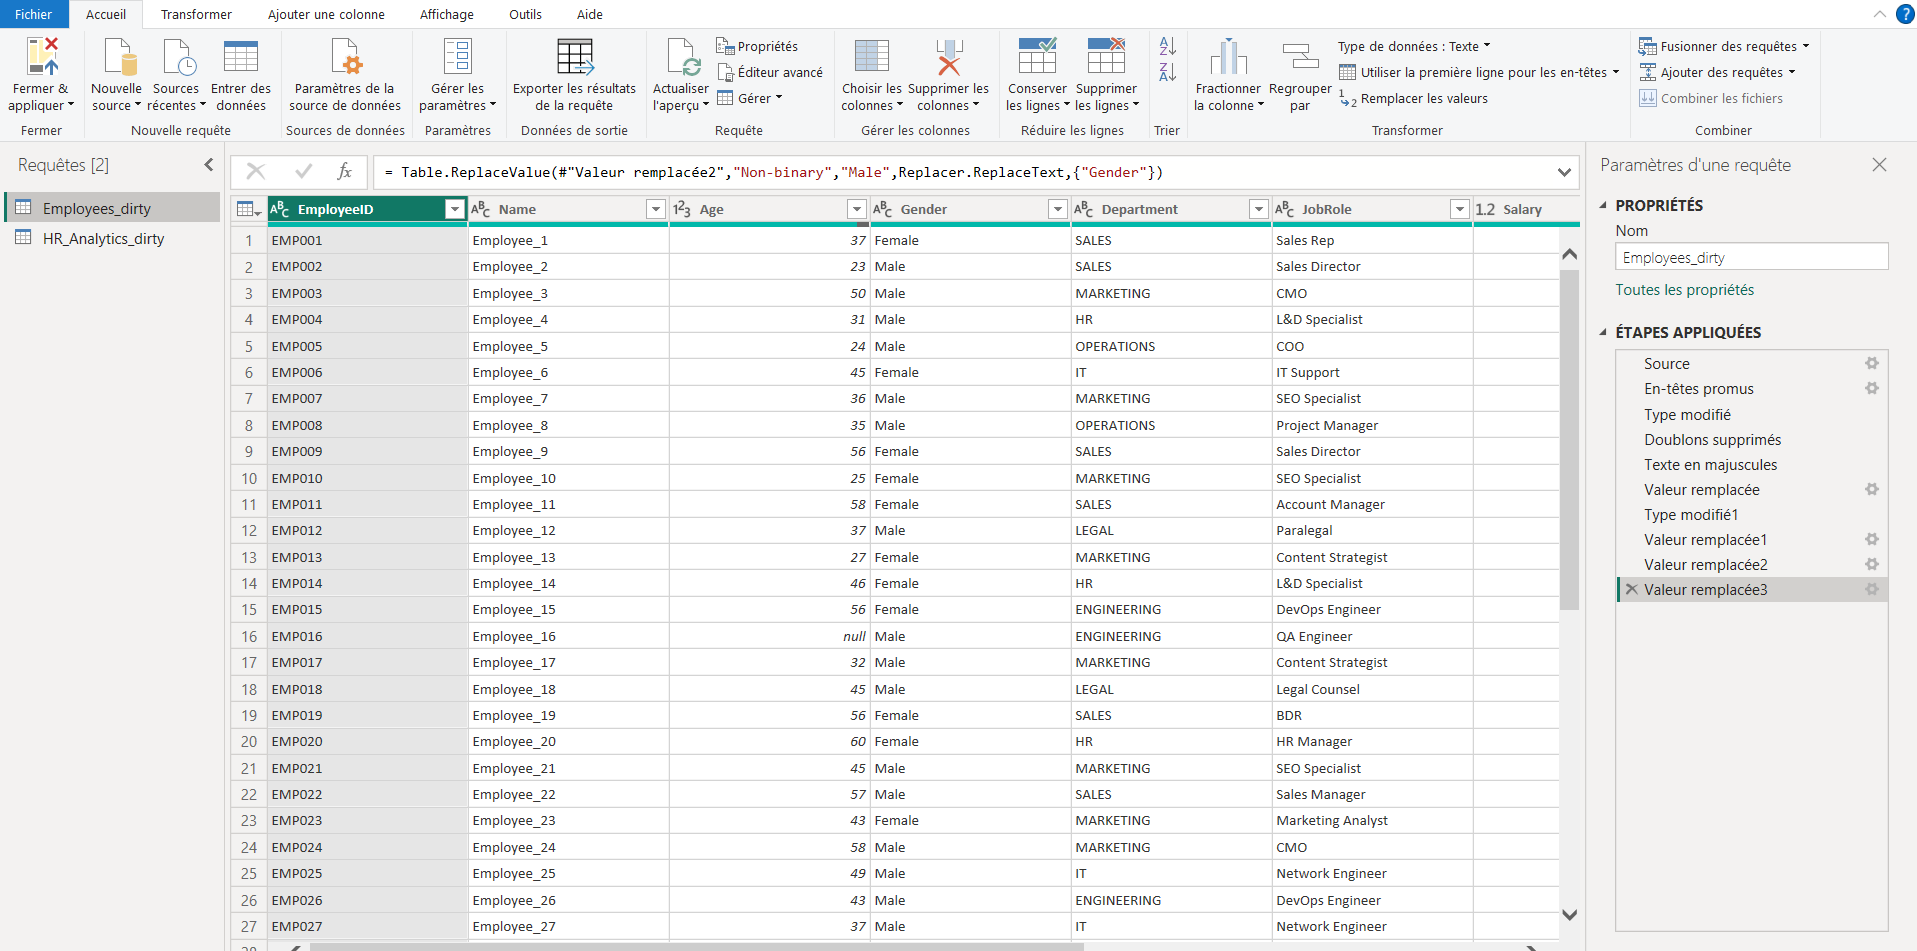
\includegraphics[width=0.8\textwidth]{figures/fig3_1_powerquery.png}
    \caption{Aperçu du pipeline de transformation Power Query}
    \label{fig:etl}
\end{figure}

\section{Modélisation Conceptuelle et Schéma en Étoile (dim\_HR.pbix)}
L'architecture du modèle repose sur un \textbf{Schéma en Étoile}, garantissant des performances optimales et une clarté analytique.

\subsection{Structure du modèle}
\begin{itemize}
    \item \textbf{FactHR (Table de faits) :} Centralise les mesures (Salaire, satisfaction, évaluation) et les clés étrangères vers les dimensions.
    \item \textbf{DimEmployee (Dimension) :} Attributs granulaires des collaborateurs (Âge, Genre, Rôle).
    \item \textbf{DimDepartment (Dimension) :} Nomenclature des pôles d'activité.
    \item \textbf{DimDate (Dimension) :} Calendrier dynamique pour les analyses temporelles.
\end{itemize}

\begin{figure}[h]
    \centering
    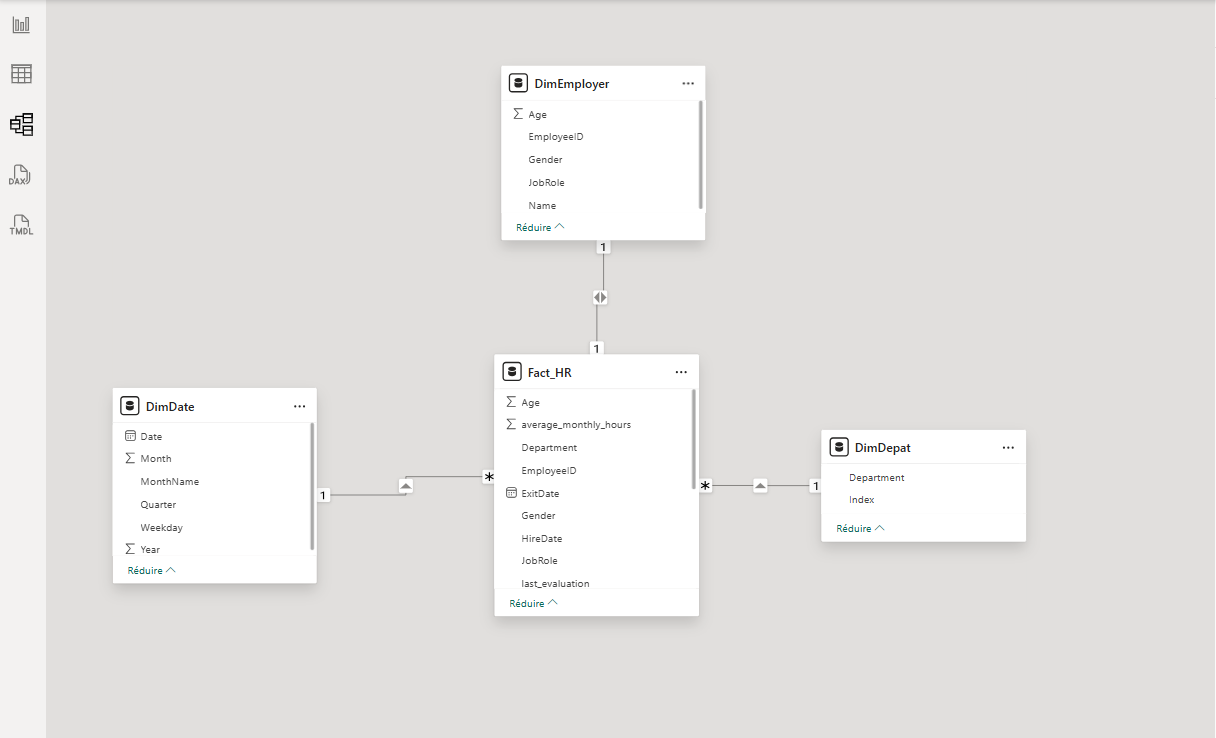
\includegraphics[width=0.9\textwidth]{figures/modele_etoile.png}
    \caption{Architecture du Schéma en Étoile finalisé}
    \label{fig:star_schema}
\end{figure}

\section{Développement des Métriques et Logique Analytique (dax\_HR.pbix)}
Le moteur DAX a été utilisé pour traduire les besoins métiers en indicateurs de performance (KPIs) dynamiques.

\subsection{Exemples de mesures DAX clés}
Nous avons implémenté des mesures avancées pour isoler les risques d'attrition :

\begin{itemize}
    \item \textbf{Attrition Rate :}
    \begin{lstlisting}[language=SQL]
Attrition Rate = 
DIVIDE(
    CALCULATE(DISTINCTCOUNT(FactHR[EmployeeID]), FactHR[left] = 1),
    [Total Employees], 0
)
    \end{lstlisting}
    
    \item \textbf{Overtime Risk Score :} Identifie les employés dépassant 220 heures mensuelles.
    \begin{lstlisting}[language=SQL]
Overtime Risk Score = 
CALCULATE(
    DISTINCTCOUNT(FactHR[EmployeeID]),
    FILTER(FactHR, FactHR[average_monthly_hours] > 220)
)
    \end{lstlisting}
\end{itemize}

\begin{figure}[h]
    \centering
    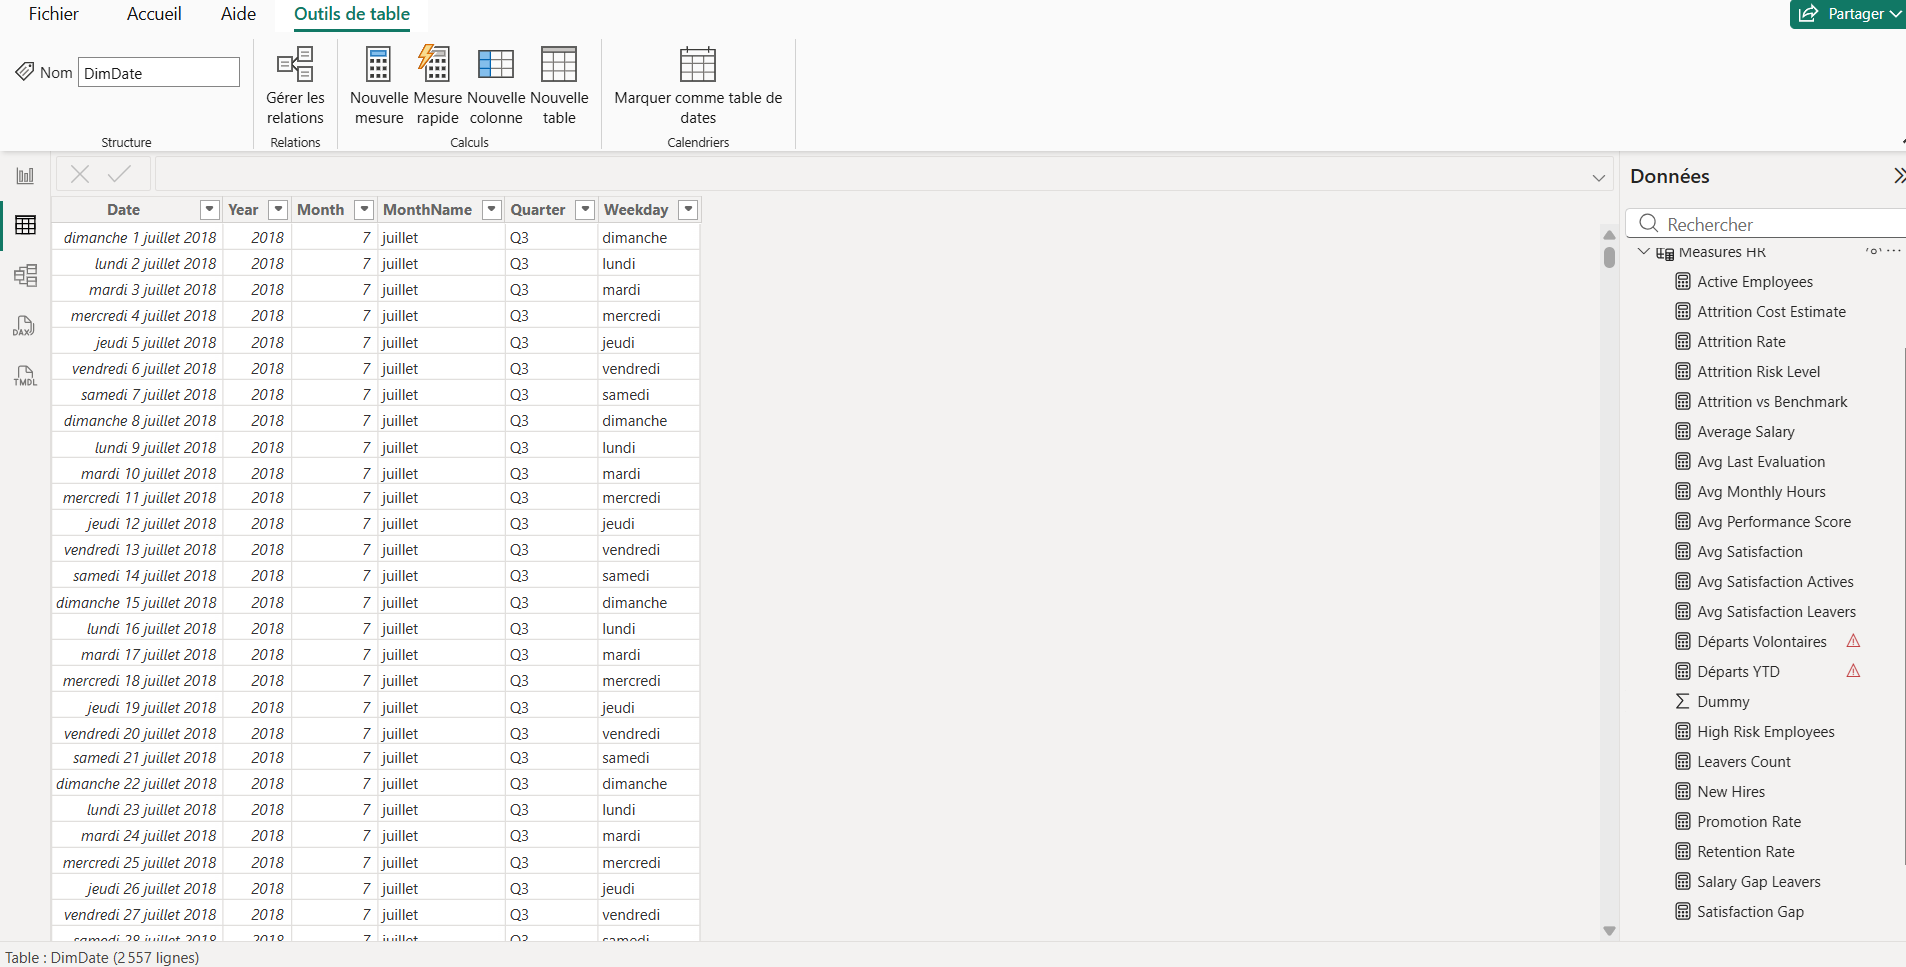
\includegraphics[width=0.8\textwidth]{figures/fig3_3_dax.png}
    \caption{Visualisation d'une mesure complexe dans Power BI Desktop}
    \label{fig:dax}
\end{figure}
